\documentclass{beamer}
\usetheme{metropolis}
\usepackage{graphicx}
\usepackage{subcaption}
\usepackage{hyperref}
\usepackage{tcolorbox}
\title{Algebra-Based Physics-1: Mechanics (PHYS135A-01): Summary}
\date{\today}
\author{Jordan Hanson}
\institute{Whittier College Department of Physics and Astronomy}

\begin{document}
\maketitle

\section{Review}

\begin{frame}{Summary}
\begin{enumerate}
\item Chapter 18 - Charges and Electric Fields
\item Chapter 19 - Electric Potential and Electric Field
\item Chapter 20 - Electric Current, Resistance, and Ohm's Law
\item Chapter 21 - Circuits and DC instruments
\item Chapter 22 - Magnetism
\item Electromagnetic Induction
\item Pivot Interactive Laboratories
\item Physics Education Technology (PhET) simulations
\item Self-designed experiments
\end{enumerate}
\end{frame}

\section{It has been my pleasure.}

\begin{frame}{Oops}
\begin{figure}

\includegraphics[width=0.85\textwidth]{savage.pdf}
\end{figure}
\end{frame}

\begin{frame}{Doctor's Visits}
\begin{figure}
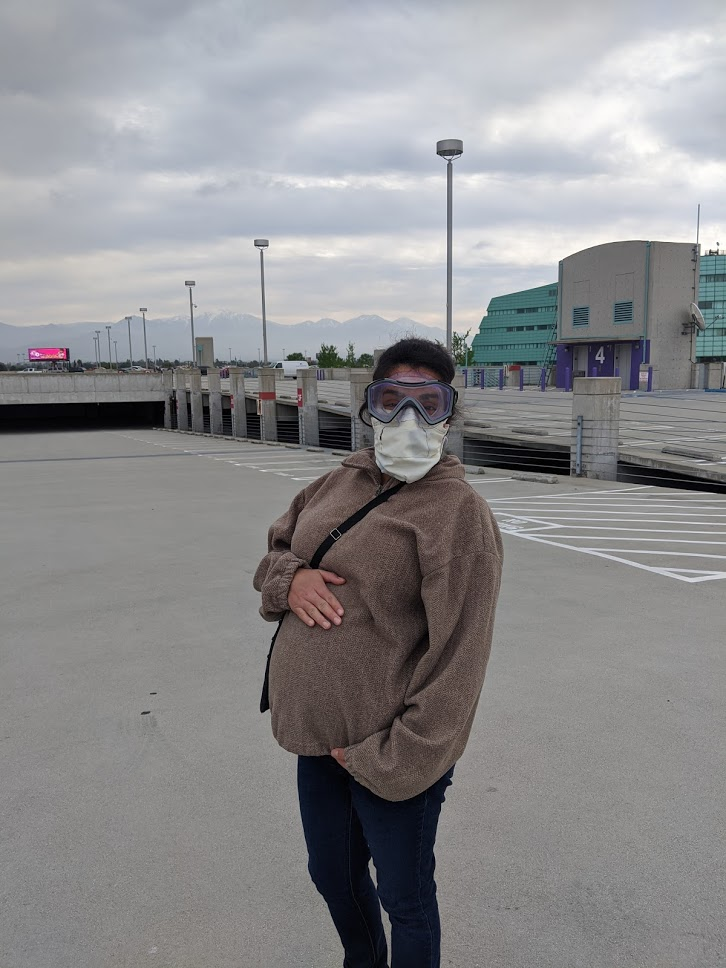
\includegraphics[width=0.5\textwidth]{priscilla1.jpg}
\end{figure}
\end{frame}

\begin{frame}{New Life}
\begin{figure}
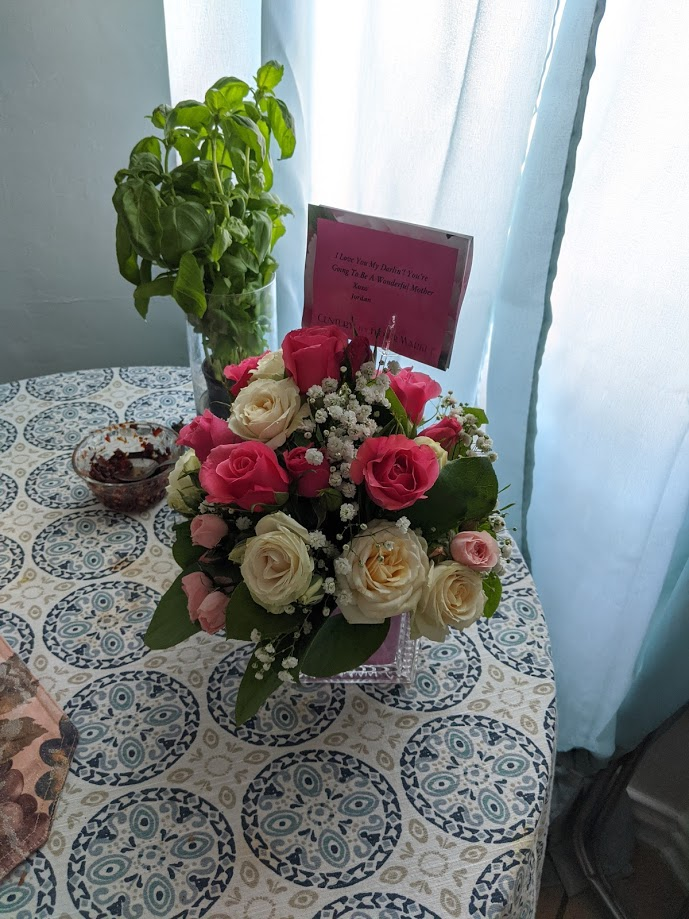
\includegraphics[width=0.5\textwidth]{flowers.jpg}
\end{figure}
\end{frame}

\begin{frame}{East Los Angeles}
\begin{figure}
\includegraphics[width=0.5\textwidth]{birth.jpg}
\end{figure}
\end{frame}

\begin{frame}{Family}
\begin{figure}
\includegraphics[width=0.4\textwidth]{wife.jpg}

\includegraphics[width=0.4\textwidth]{green.jpg}
\end{figure}
\end{frame}

\begin{frame}{Birthday}
\begin{figure}
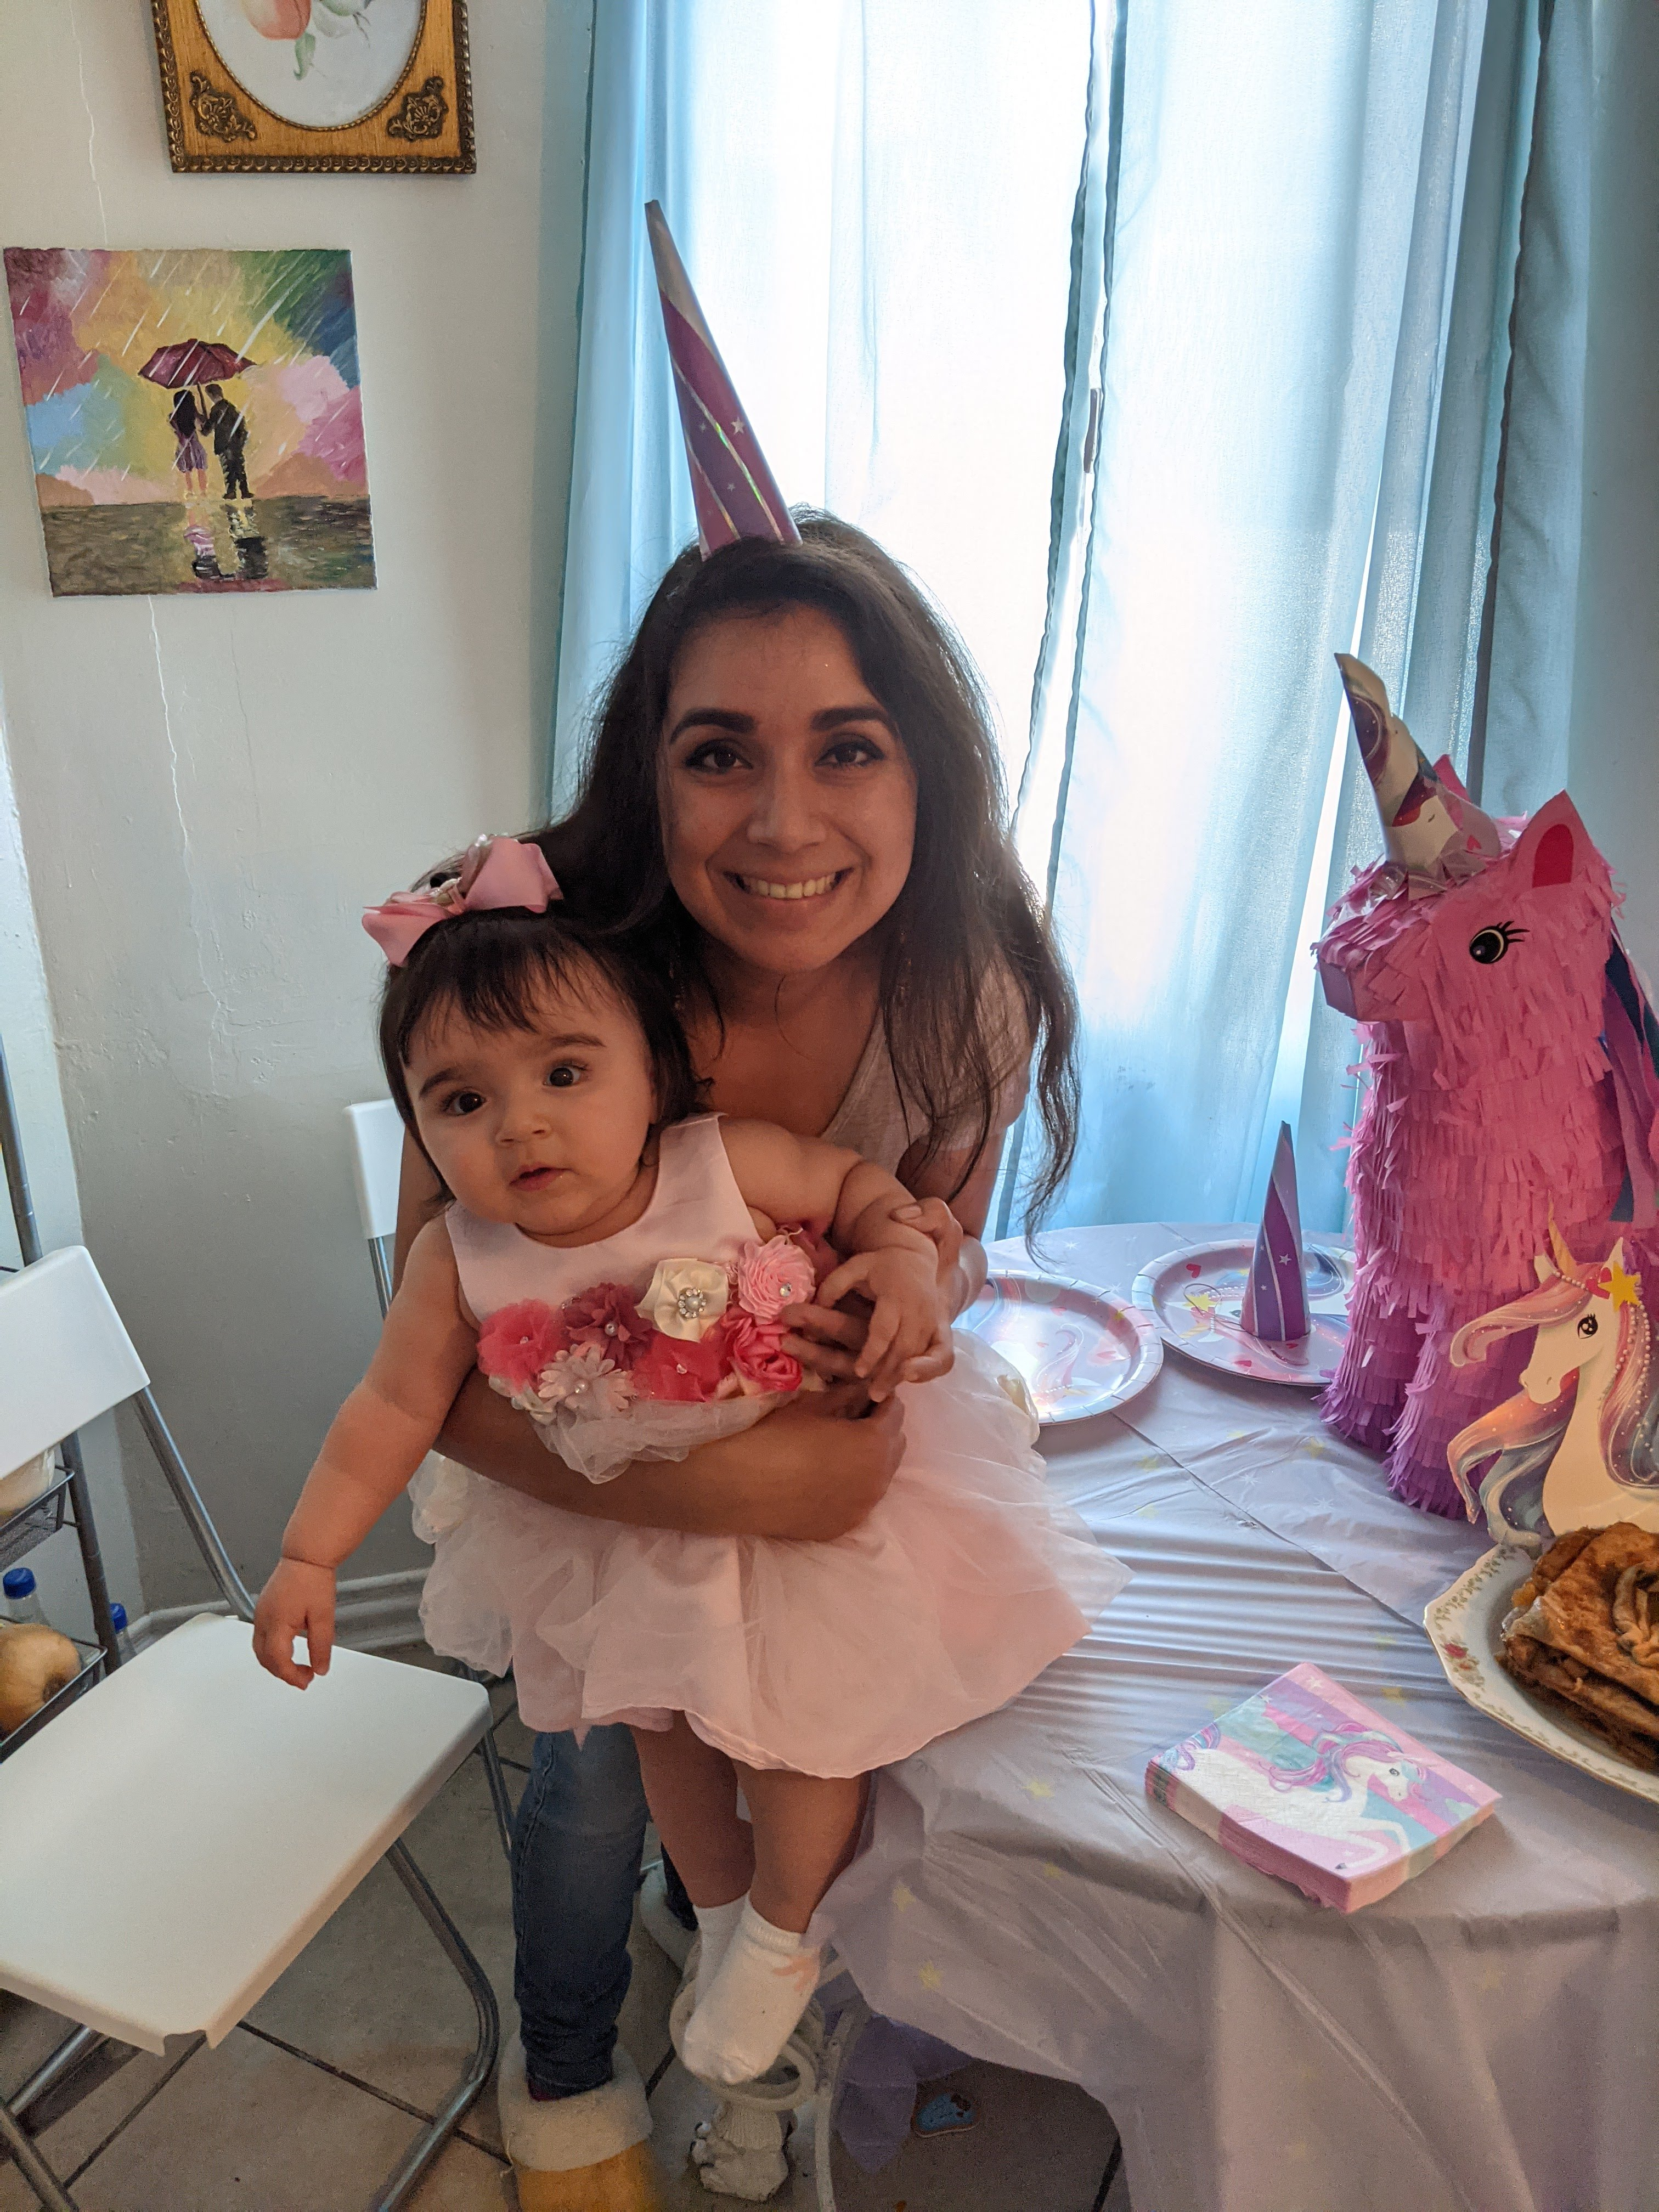
\includegraphics[width=0.5\textwidth]{bday.jpg}
\end{figure}
\end{frame}

\begin{frame}{Work}
\begin{figure}
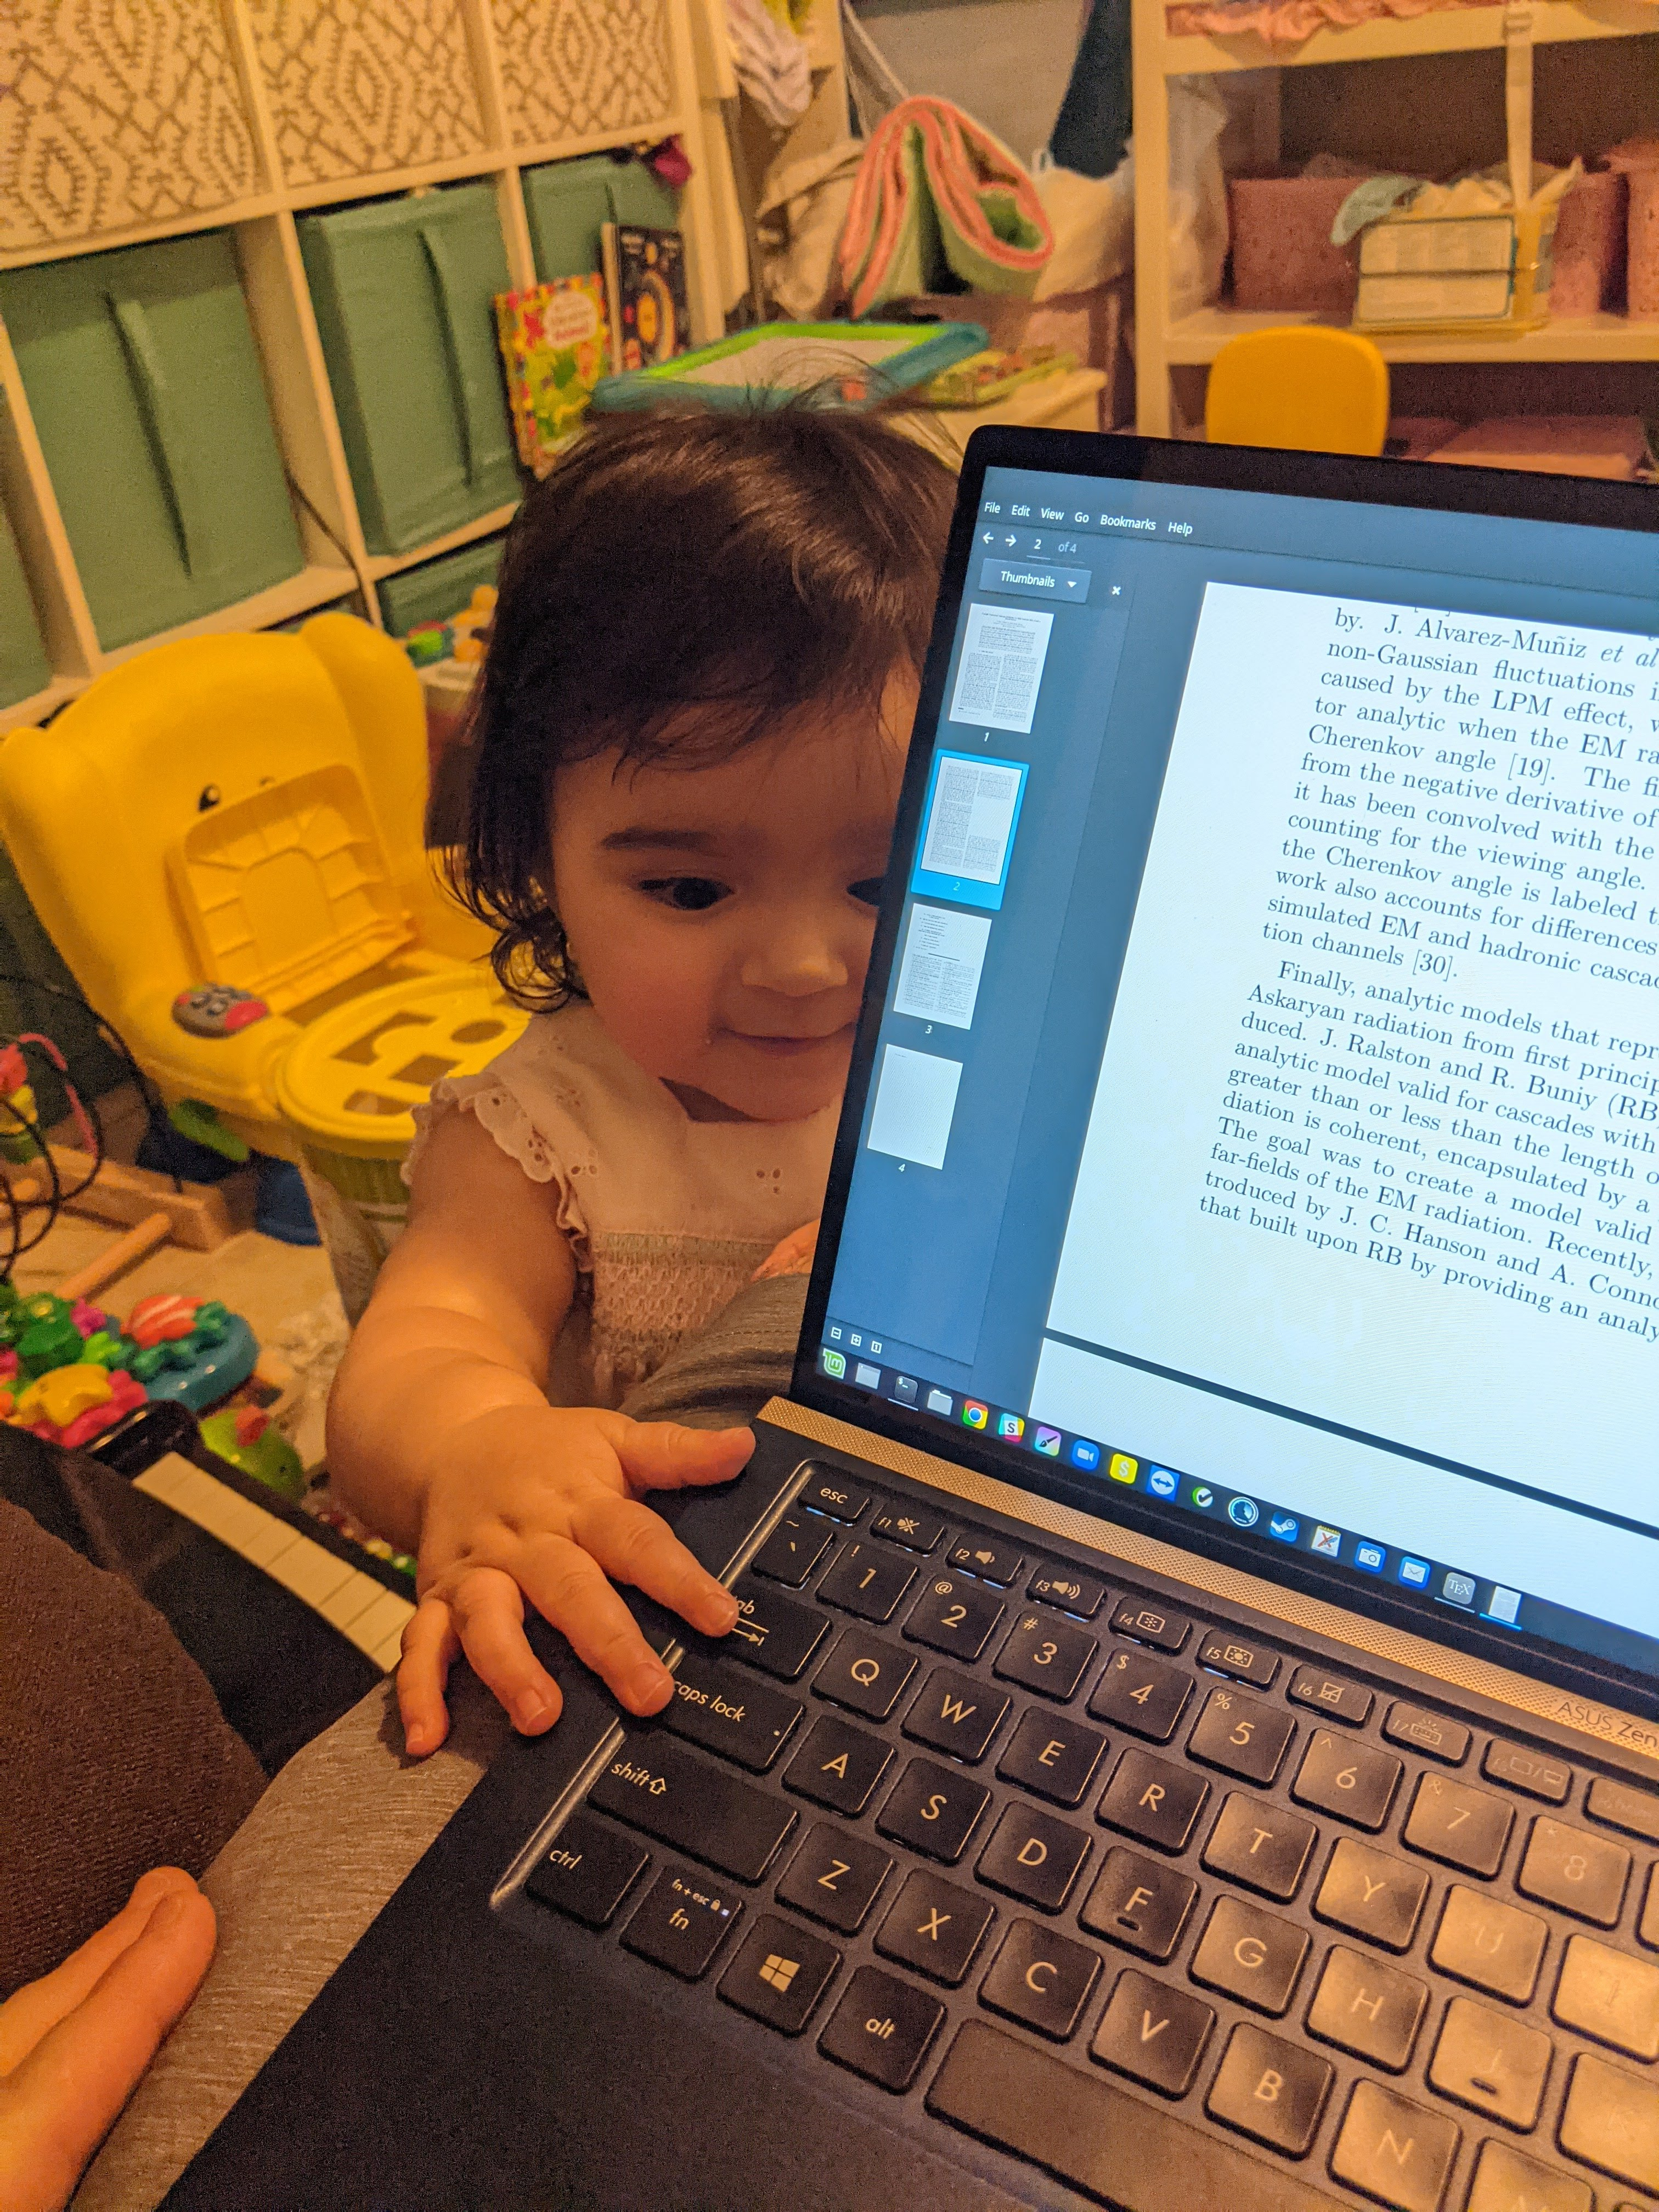
\includegraphics[width=0.5\textwidth]{work.jpg}
\end{figure}
\end{frame}

\begin{frame}{Sleep}
\begin{figure}
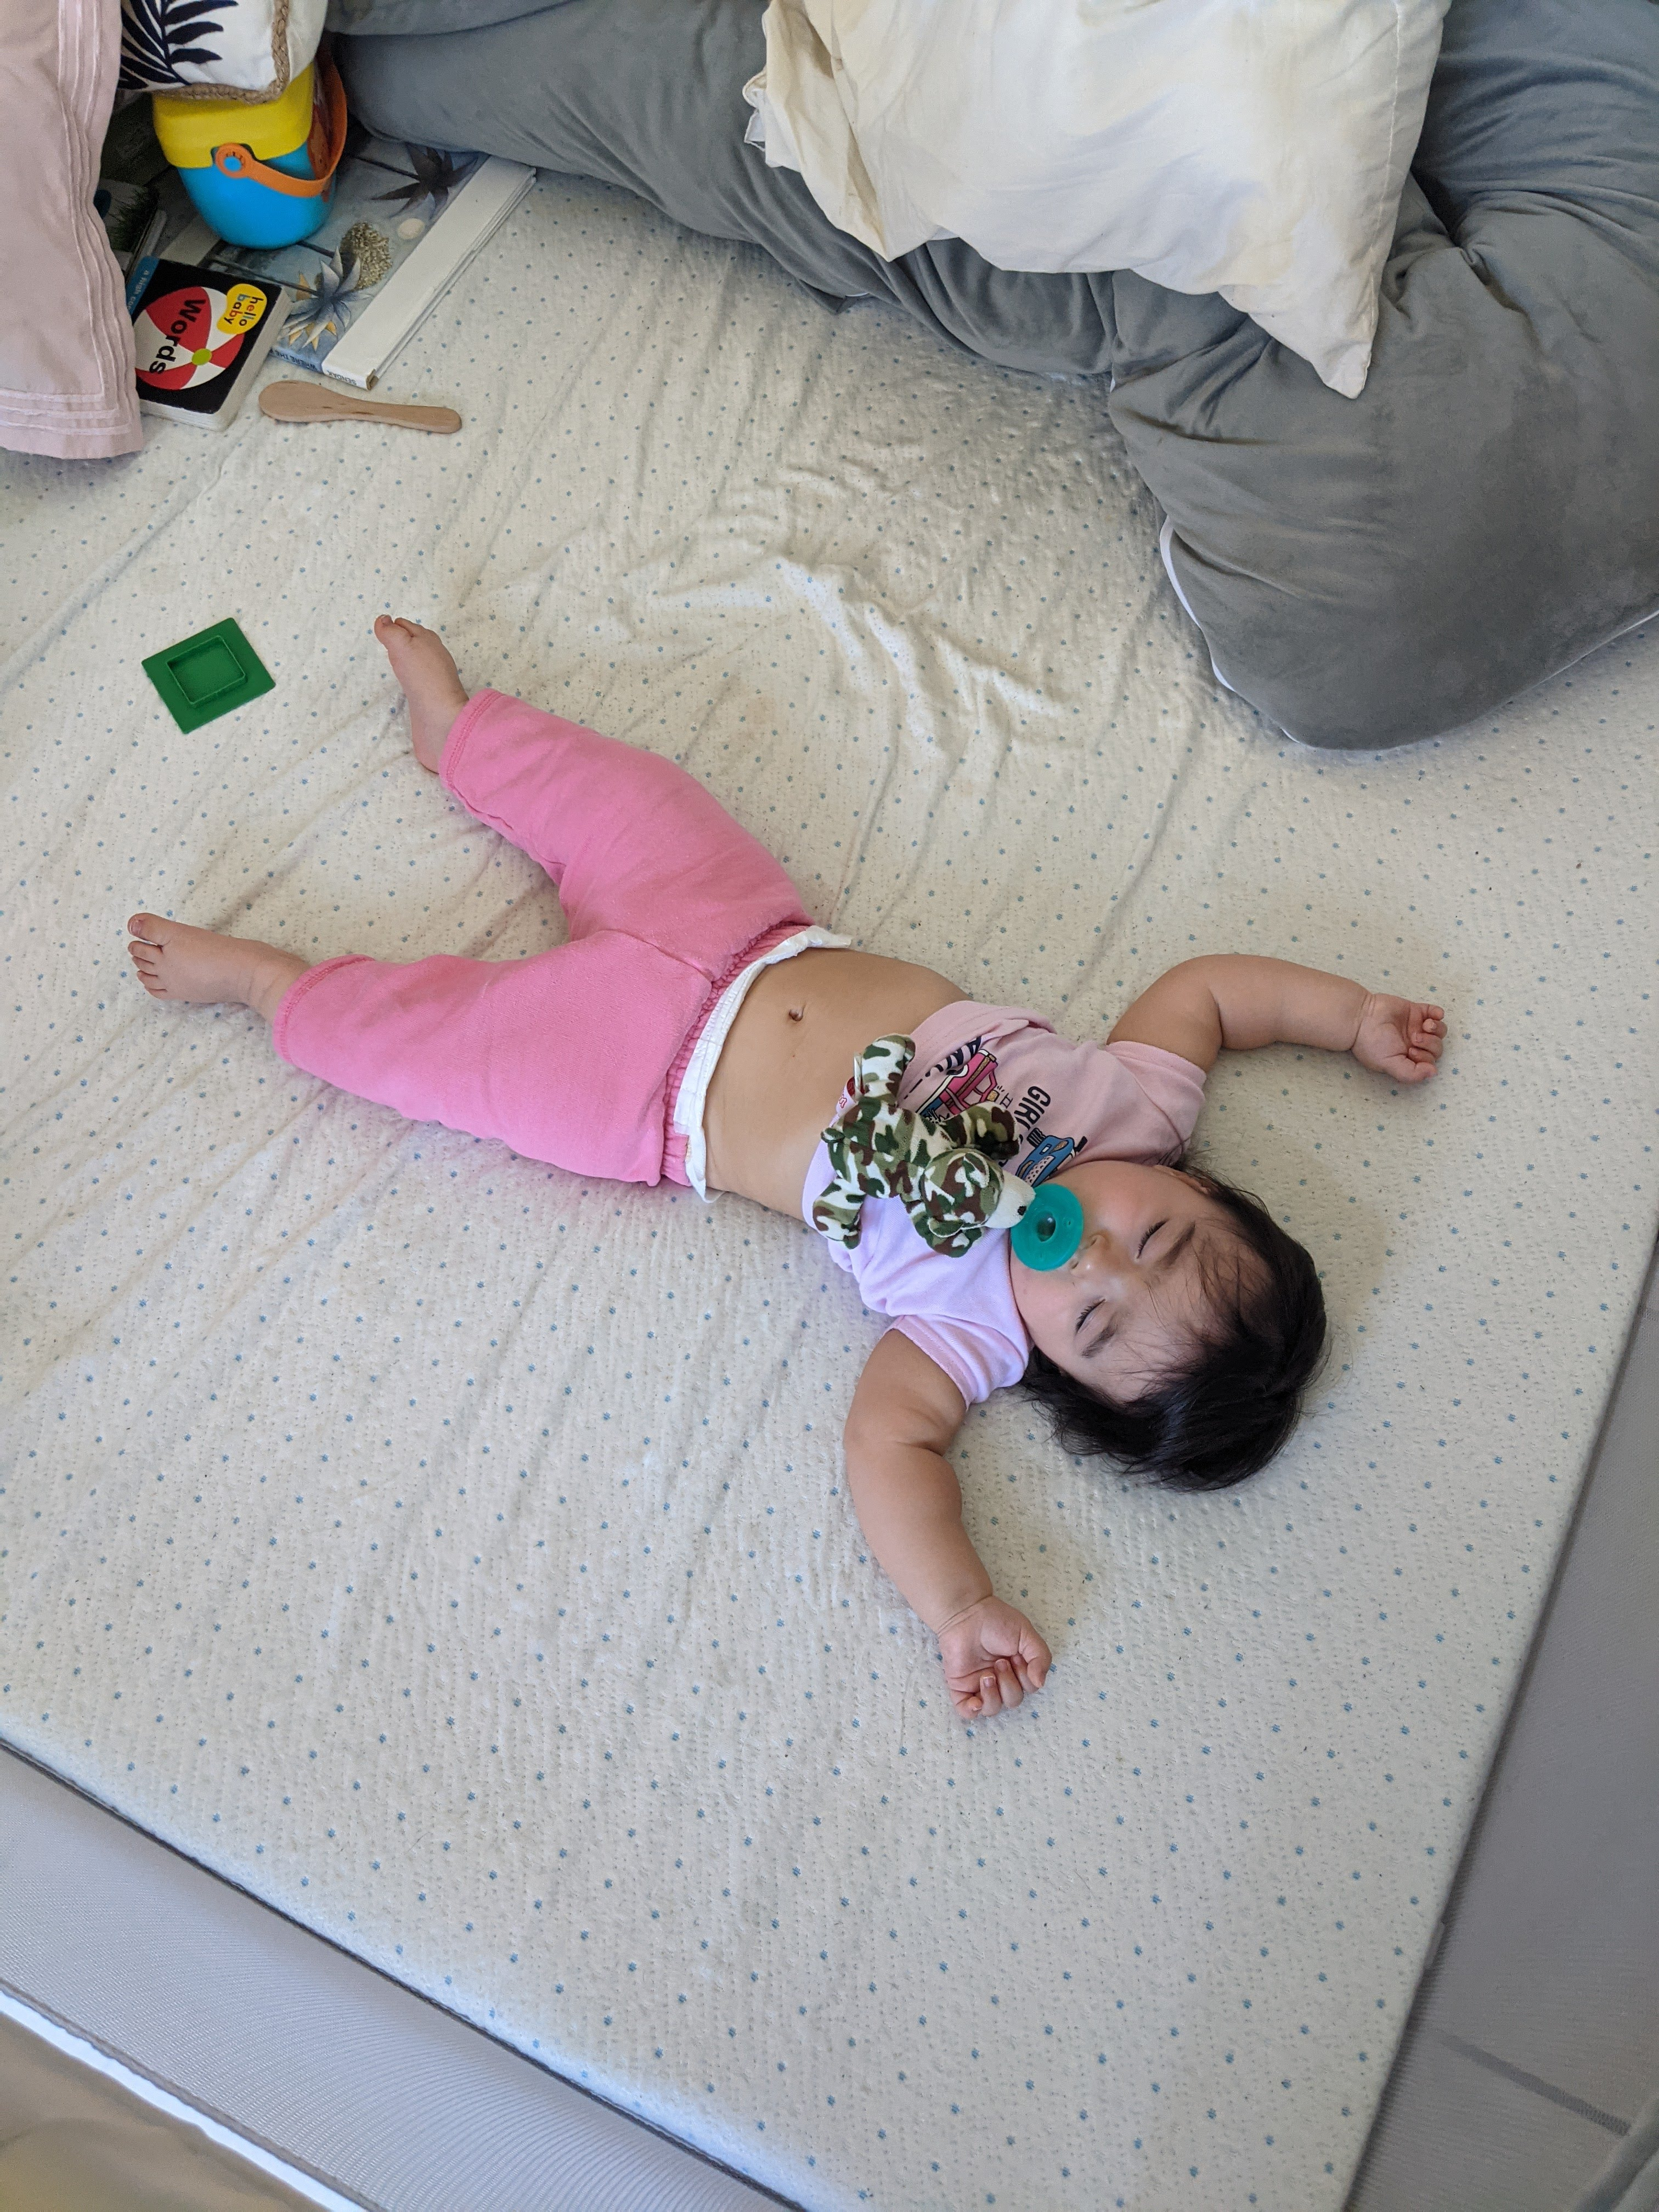
\includegraphics[width=0.5\textwidth]{sleep.jpg}
\end{figure}
\end{frame}

\begin{frame}{Whittier College}
\begin{figure}
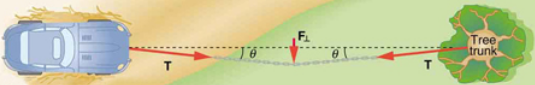
\includegraphics[width=0.5\textwidth]{tree.jpg}
\end{figure}
\end{frame}

\section{Thank you.}

\end{document}
